\documentclass[12pt]{article}
\usepackage[paperwidth=9.6in,paperheight=12.8in,margin=0.18in]{geometry}
\usepackage[T1]{fontenc}
\usepackage{lmodern}
\usepackage{amsmath}
\usepackage{xcolor}
\usepackage{tikz}
\usetikzlibrary{arrows.meta,positioning,shapes.geometric}

\definecolor{psidblue}{HTML}{1E3A5F}
\definecolor{psidline}{HTML}{D1D5DB}
\definecolor{psidpanel}{HTML}{F7FAFC}
\definecolor{psidaccent}{HTML}{E8F1FB}
\definecolor{psidgold}{HTML}{A16207}

\pagestyle{empty}
\setlength{\parindent}{0pt}
\setlength{\parskip}{0pt}

\tikzset{
  flowstep/.style={
    rectangle,
    rounded corners=6pt,
    draw=psidblue,
    fill=psidpanel,
    very thick,
    align=center,
    text width=3.6cm,
    minimum height=1cm,
    font=\sffamily\small
  },
  flowwide/.style={flowstep, text width=4.4cm},
  flowresult/.style={flowstep, draw=psidgold!85!black, fill=psidaccent},
  flowarrow/.style={-{Stealth[length=3mm]}, very thick, draw=psidblue}
}

\begin{document}
\thispagestyle{empty}
\centering
\resizebox{0.96\textwidth}{!}{%
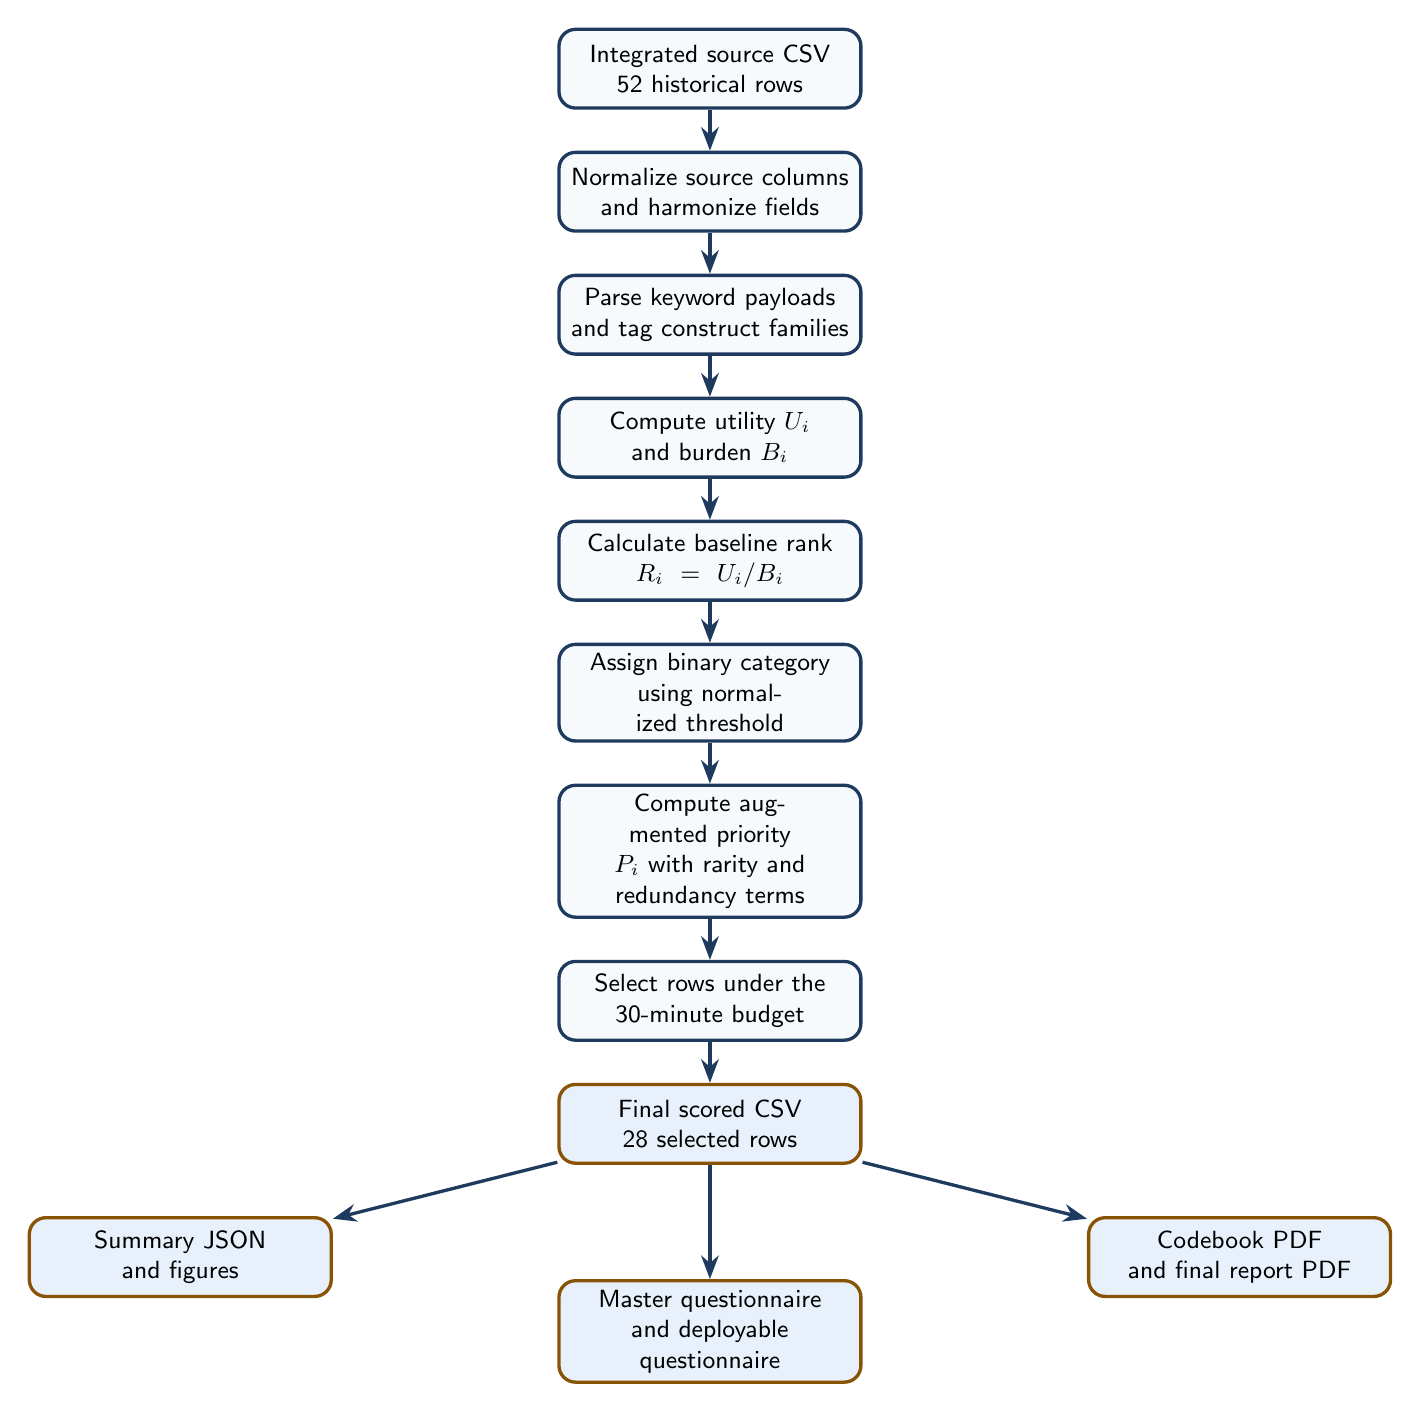
\begin{tikzpicture}[node distance=0.52cm]
\node[flowstep] (a) {Integrated source CSV\\52 historical rows};
\node[flowstep, below=of a] (b) {Normalize source columns\\and harmonize fields};
\node[flowstep, below=of b] (c) {Parse keyword payloads\\and tag construct families};
\node[flowstep, below=of c] (d) {Compute utility $U_i$\\and burden $B_i$};
\node[flowstep, below=of d] (e) {Calculate baseline rank\\$R_i = U_i / B_i$};
\node[flowstep, below=of e] (f) {Assign binary category\\using normalized threshold};
\node[flowstep, below=of f] (g) {Compute augmented priority\\$P_i$ with rarity and redundancy terms};
\node[flowstep, below=of g] (h) {Select rows under the\\30-minute budget};
\node[flowresult, below=of h] (i) {Final scored CSV\\28 selected rows};
\node[flowresult, below left=0.65cm and 2.85cm of i] (j) {Summary JSON\\and figures};
\node[flowresult, below=1.45cm of i] (k) {Master questionnaire\\and deployable questionnaire};
\node[flowresult, below right=0.65cm and 2.85cm of i] (l) {Codebook PDF\\and final report PDF};
\draw[flowarrow] (a) -- (b);
\draw[flowarrow] (b) -- (c);
\draw[flowarrow] (c) -- (d);
\draw[flowarrow] (d) -- (e);
\draw[flowarrow] (e) -- (f);
\draw[flowarrow] (f) -- (g);
\draw[flowarrow] (g) -- (h);
\draw[flowarrow] (h) -- (i);
\draw[flowarrow] (i) -- (j);
\draw[flowarrow] (i) -- (k);
\draw[flowarrow] (i) -- (l);
\end{tikzpicture}
}
\end{document}